\thispagestyle{plain}
\chapter{Θεωρητικό Υπόβαθρο και Εργαλεία}
\label{chap:3}

\section{Θεωρητικό Υπόβαθρο}
\label{sec:3.1}

\subsection{Βασικοί ορισμοί}
\label{subsec:3.1.1}

Με τον όρο \textit{Τεχνητή Νοημοσύνη - Artificial Intelligence} περιγράφεται η ικανότητα των μηχανών να μιμούνται ορισμένες λειτουργίες του ανθρώπινου εγκεφάλου όπως  μάθηση, προσαρμοστικότητα, εξαγωγή συμπερασμάτων, κατανόηση από συμφραζόμενα, επίλυση προβλημάτων κα.

 Η \textit{Μηχανική Μάθηση - Machine Learning} είναι υποσύνολο της Τεχνητής Νοημοσύνης και αποτελεί πεδίο μελέτης στο οποίο δίνεται η ικανότητα στους υπολογιστές να μαθαίνουν, χωρίς να έχουν προγραμματιστεί ρητά για την εκάστοτε λειτουργία. 
 
Μία από τις ευρέως γνωστές εργασίες Μηχανικής Μάθησης αποτελεί η \textit{Επιβλεπόμενη Μάθηση - Supervised Learning}. Στους αλγόριθμους Επιβλεπόμενης Μάθησης δίνεται ένα σύνολο δεδομένων και η επιθυμητή έξοδος. Ο αλγόριθμος προσπαθεί να εντοπίσει τις συσχετίσεις μεταξύ εισόδου και εξόδου. Μετά την εκπαίδευση, δηλαδή την προσπάθεια εύρεσης των συσχετίσεων εισόδου-εξόδου, δημιουργείται ένα μοντέλο το οποίο αναμένεται να μπορεί να προβλέπει την έξοδο για νέα δεδομένα στην είσοδο. Το μοντέλο πρέπει να γενικεύει αρκετά και όχι να ‘αποστηθίζει’ τα δεδομένα στα οποία εκπαιδεύτηκε, διαφορετικά δεν θα μπορεί να προβλέψει σωστά την έξοδο για νέες εισόδους. 


Επιγραμματικά, οι σημαντικότεροι αλγόριθμοι Επιβλεπόμενης Μάθησης είναι οι εξής: Τεχνητά Νευρωνικά Δίκτυα(Artificial Neural Networks), Μηχανές Διανυσμάτων Υποστήριξης(Support Vector Machines), Γραμμική Παλινδρόμηση(Linear Regression), Λογιστική Παλινδρόμηση(Logistic Regression), Δίκτυα Bayes(Naive Bayes), Γραμμική Διακριτική Ανάλυση(Linear Discriminant Analysis), Δέντρα Απόφασης(Decision Trees), Κ - κοντινότεροι Γείτονες(K-nearest Neighbor) και Εκμάθηση με μέτρο ομοιότητας(Similarity learning). 


\subsection{Τεχνητά Νευρωνικά Δίκτυα(Artificial Neural Network)}
\label{subsec:3.1.2}


Τα Τεχνητά Νευρωνικά Δίκτυα είναι υπολογιστικά συστήματα εμπνευσμένα  από βιολογικά νευρικά δίκτυα τα οποία συνιστούν τον εγκέφαλο των ζώων.  Αποτελούνται από επίπεδα
με συνδεδεμένους κόμβους που ονομάζονται νευρώνες ενώ οι συνδέσεις ανάμεσα στους νευρώνες ονομάζονται ακμές. Οι νευρώνες ενός επιπέδου είναι συνδεδεμένοι με όλους ή κάποιους από τους νευρώνες του προηγούμενου και του επόμενου επιπέδου.


Κάθε νευρώνας δέχεται ένα σύνολο αριθμητικών εισόδων είτε από άλλους νευρώνες, είτε από το περιβάλλον, με βάση αυτές τις εισόδους εκτελεί έναν υπολογισμό και παράγει μία έξοδο. Στην εικόνα \ref{figure:basicann} παρουσιάζεται μία απλή δομή ANN με τρία επίπεδα: το επίπεδο εισόδου(Input Layer), το κρυμμένο επίπεδο(Hidden Layer) και το επίπεδο εξόδου(Output Layer). Ωστόσο, σε μία πιο σύνθετη μορφή συναντάμε περισσότερα από ένα κρυφά επίπεδα. Επίσης, δεν υπάρχει περιορισμός στον αριθμό των νευρώνων σε κάθε επίπεδο.



\begin{figure}[!h]
    \centering
      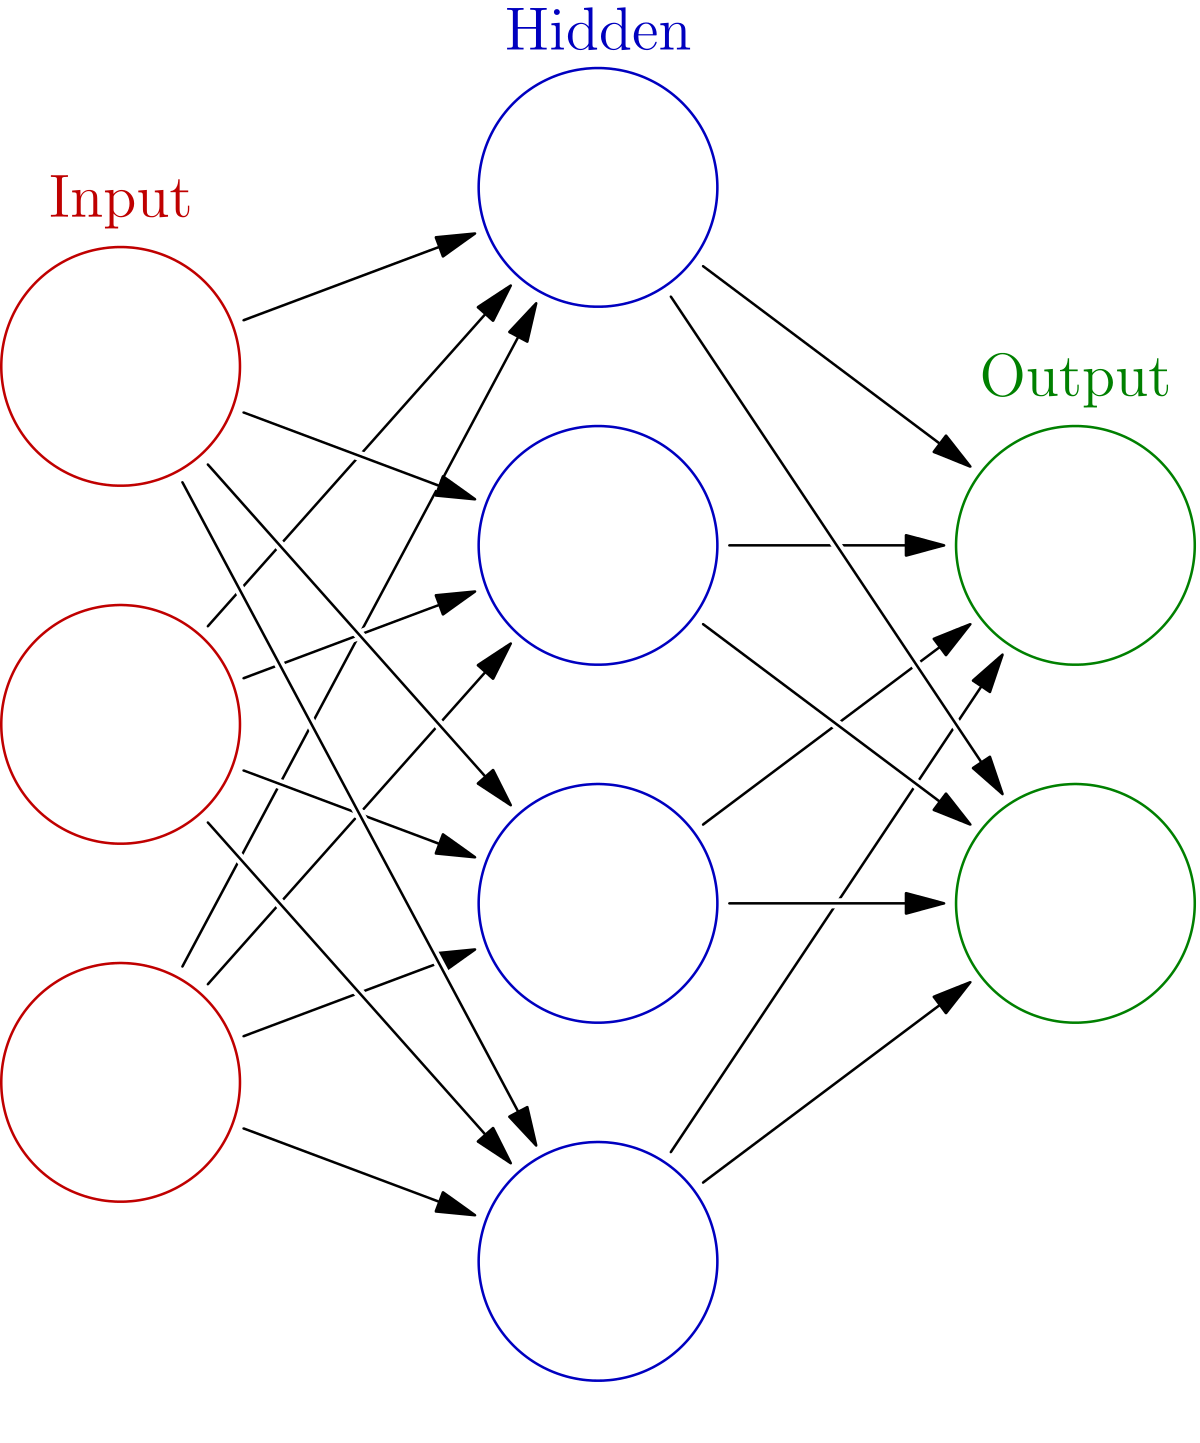
\includegraphics[width=0.3\linewidth]{basic_ann.png} \caption{Βασική δομή ANN}
          \label{figure:basicann}  

  \end{figure}



Ένα ANN μπορεί να περιγραφεί ως ένας κατευθυνόμενος γράφος που κάθε κόμβος $i$ εκτελεί μία συνάρτηση μεταφοράς $f_{i}$ της μορφής: \cite{Yao}




\begin{equation} \label{eq:1}
y_{i} = f_{i}(\sum_{j=1}^{n}w_{ij}x_{j}+\theta_{i})
\end{equation}


όπου $y_{i}$ είναι η έξοδος του κόμβου $i$, $x_{j}$ είναι η $j^{th}$ είσοδος στο $i$ κόμβο, $w_{ij}$ είναι το βάρος που συνδέει τους κόμβους $i$ και $j$ και $θ_{i}$(ή bias) είναι το κατώφλι του κόμβου μέσω του οποίου μπορεί να ρυθμιστεί περαιτέρω η ενεργοποίηση του νευρώνα. Η συνάρτηση $f_{i}$ είναι συνήθως μη γραμμική και ονομάζεται συνάρτηση ενεργοποίησης. Κάποιες συνηθισμένες μορφές της είναι οι \ref{eq:Rectifier}, \ref{eq:Sigmoid}, \ref{eq:tanh}.

Ανόρθωσης(Rectifier): 
\begin{equation} \label{eq:Rectifier}
φ(x) = max(0, x)
\end{equation}
\\


Λογιστική σιγμοειδής(Logistic Sigmoid): 
\begin{equation} \label{eq:Sigmoid}
φ(x) = \frac{1}{1+ e^{-x}}
\end{equation}
\\


Υπερβολική εφαπτομένη(Hyperbolic tangent): 
\begin{equation} \label{eq:tanh}
φ(x) = tanh(x)
\end{equation}

Ξεχωριστό ρόλο επιτελούν οι νευρώνες εισόδου, οι οποίοι δεν επιτελούν κάποιο υπολογισμό αλλά αναλαμβάνουν να τροφοδοτήσουν το δίκτυο με την είσοδο και οι νευρώνες εξόδου που διοχετεύουν στο περιβάλλον τις τελικές αριθμητικές εξόδους του δικτύου.

 
Το ANN μετά από μία διαδικασία που ονομάζεται εκπαίδευση θα πρέπει να μπορεί να προβλέπει την έξοδο, για νέες εισόδους. Η εκπαίδευση περιλαμβάνει τη σωστή ρύθμιση των βαρών και του κατωφλίου που αναφέρθηκαν στην \ref{eq:1}, σε τιμές κατάλληλες ώστε να επιλύεται με επαρκή επιτυχία το προς εξέταση πρόβλημα. Αυτό γίνεται με μία διαδικασία ανάδρασης που ονομάζεται backpropagation.


Αρχικά, τα δεδομένα περνάνε από όλα τα επίπεδα και υπολογίζεται η πρόβλεψη του δικτύου. Στη συνέχεια, συγκρίνεται η πραγματική κλάση στην οποία ανήκουν τα δεδομένα με την πρόβλεψη του δικτύου και υπολογίζεται το διάνυσμα σφάλματος. Τέλος, το διάνυσμα σφάλματος ανατροφοδοτείται διαδοχικά στα προηγούμενα επίπεδα, από το επίπεδο εξόδου στο επίπεδο εισόδου, και οι νευρώνες κάθε επιπέδου αναπροσαρμόζουν τις παραμέτρους προς την κατεύθυνση μείωσης του σφάλματος. Αφού το δίκτυο εκπαιδευτεί, τα βάρη και η παράμετρος κατωφλίου παγώνουν και πια το μοντέλο είναι έτοιμο να κάνει προβλέψεις για νέες εισόδους διαφορετικές από αυτές στις οποίες εκπαιδεύτηκε.
    




\subsection{Συνελικτικά Νευρωνικά Δίκτυα(Convolutional Neural Network)}
\label{subsec:3.1.3}



Προηγουμένως, έγινε μια συνοπτική ανάλυση των ANN ώστε να τεθούν οι βάσεις για την περιγραφή των \textit{Συνελικτικών Νευρωνικών Δικτύων} τα οποία χρησιμοποιούνται στην παρούσα διπλωματική. Τα \textit{Συνελικτικά Νευρωνικά Δίκτυα} είναι μία ευρέως χρησιμοποιούμενη αρχιτεκτονική της Μηχανικής Μάθησης και αποτελεί κατηγορία των Τεχνητών Νευρωνικών Δικτύων.
Αποτελούνται από ένα ή περισσότερα επίπεδα συνέλιξης, ακολουθούμενα συνήθως από επίπεδα υποδειγματοληψίας. Τα τελευταία επίπεδα του δικτύου συνήθως περιέχουν πλήρη συνδεδεμένα επίπεδα για την ταξινόμηση των εισόδων στις κλάσεις.
Η περιγραφή των παραπάνω επιπέδων θα δοθεί σε επόμενες παραγράφους.


Συνοπτικά, η λειτουργιά των CNN μπορεί να περιγραφεί ως εξής: Αρχικά, οι εικόνες εισόδου διέρχονται από τα διάφορα επίπεδα και το νευρωνικό  εξάγει σταδιακά όλο και πιο σύνθετα τοπικά χαρακτηριστικά μέσω της προσαρμογής των διαφόρων φίλτρων των συνελικτικών επιπέδων. Στα πρώτα συνελικτικά επίπεδα το δίκτυο μαθαίνει κάποιες απλές δομές ενώ σε μεγαλύτερο βάθος εξάγονται πιο σύνθετα χαρακτηριστικά. Για παράδειγμα, αν η είσοδος  είναι μία εικόνα, στα πρώτα επίπεδα εξάγονται ακμές και βασικά σχήματα ενώ σε υψηλότερα επίπεδα μπορεί να εξαχθούν σύνθετες δομές, για παράδειγμα ψηφία, γράμματα και πρόσωπα. Έπειτα, τα χαρακτηριστικά που εξήχθησαν αντιστοιχίζονται στους χάρτες χαρακτηριστικών(feature maps) που αποτελούν μια βιβλιοθήκη των χαρακτηριστικών  που εμφανίζονται στις εικόνες μιας κλάσης. Μέσω της παραπάνω αντιστοίχισης είναι δυνατή η πρόβλεψη της εξόδου για νέες εικόνες στην είσοδο. Στην εικόνα \ref{figure:convNet} παρουσιάζεται μία τυπική δομή ενός συνελικτικού δικτύου.




\begin{figure}[!h]
    \centering
      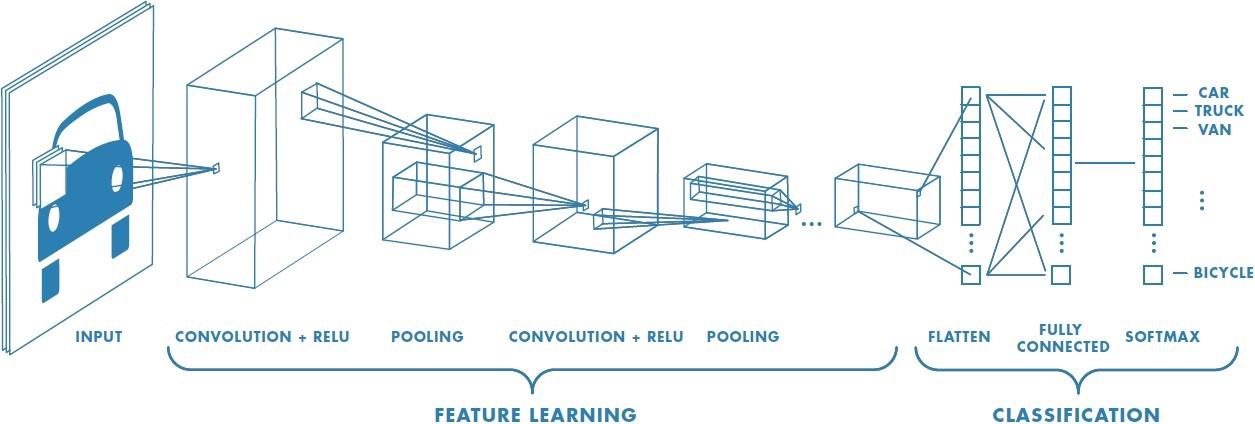
\includegraphics[width=0.95\linewidth]{convNet.jpeg} \caption{Τυπική δομή ενός Συνελικτικού Δικτύου}
      \label{figure:convNet}    
  \end{figure}


Τα Συνελικτικα Νευρωνικα Δικτυα προτιμουνται έναντι των Πλήρως Συνδεδεμένων Δικτύων, δηλαδή των δικτύων στα οποία οι νευρώνες ενός επιπέδου είναι συνδεδεμένοι με όλους τους νευρώνες του προηγούμενου και του επόμενου επιπέδου, λόγω του μικρότερου αριθμού παραμέτρων που απαιτούν. Για παράδειγμα, ένα πλήρως συνδεδεμένο δίκτυο για μία μικρή εικόνα 200x200 απαιτεί 40000 παραμέτρους για κάθε νευρώνα στο επόμενο επίπεδο. Εν αντιθέσει, ένα συνελικτικό επίπεδο περιέχει σταθερά φίλτρα διαφόρων διαστάσεων ανεξάρτητα από την είσοδο. Το Νευρωνικά Συνελικτικά Δίκτυα αποτελούνται από διάφορα δομικά στοιχεία τα οποία τελούν διαφορές λειτουργιές. Παρακάτω γίνεται μια συνοπτική παρουσίαση μερικών σημαντικών δομικών στοιχείων που εμφανίζονται στα Συνελεκτικό Δίκτυα και συγκεκριμένα στο Inception V3, το οποίο χρησιμοποιήθηκε στην παρούσα διπλωματική.


\subsubsection{Συνελικτικο Επίπεδο(Convolutional Layer)}
\label{subsubsec:3.1.3.1}


Ένα συνελικτικό επίπεδο περιέχει φίλτρα των οποίων οι τιμές καθορίζονται κατά την εκπαίδευση. Τα φίλτρα συνεχίζονται με την είσοδο και παράγονται οι χάρτες χαρακτηριστικών, οι οποίοι περιέχουν τις θέσεις ενεργοποίησης των φίλτρων. Ουσιαστικά το φίλτρο ολισθαίνει πάνω στην είσοδο και το αποτέλεσμα της συνέλιξης σε μία συγκεκριμένη χωρική θέση της εισόδου υπολογίζεται ως το γινόμενο(στοιχείο προς στοιχείο) του φίλτρου και ενός παραθύρου της εικόνας ίδιων διαστάσεων με το φίλτρο και με κεντρικό εικονοστοιχείο το σημείο στη συγκεκριμένη χωρική θέση. Οι διαστάσεις των φίλτρων(ύψος και πλάτος), πρέπει να είναι μικρότερες από αυτές της εικόνας.
 
 
Έτσι, για μία εικόνα MxNxC όπου MxN το ύψος και πλάτος της εικόνας αντίστοιχα και C ο αριθμός των καναλιών της, η συνέλιξη με C1 φίλτρα M1xN1 θα δώσει ως αποτέλεσμα χάρτες χαρακτηριστικών με διαστάσεις (Μ-Μ1+1)x(N-N1+1)xC1. Όπως είναι φανερό το ύψος και το πλάτος της εικόνας θα μειωθούν ανάλογα με το ύψος και το πλάτος του φίλτρου συνέλιξης. Η μείωση αυτή οφείλεται στα άκρα της εικόνες καθώς για να είναι δυνατή η συνέλιξη σε μία θέση της εικόνας θα πρέπει να υπάρχουν οι αντίστοιχοι γείτονες για να πολλαπλασιαστεί το φίλτρο. Επίσης, ο αριθμός των καναλιών αλλάζει από C σε C1. Η αλλαγή αυτή προκύπτει καθώς τα C1 φίλτρα διάστασης M1xN1 στην πραγματικότητα είναι C1 φίλτρα διάστασης M1xN1xC.




Στην \ref{figure:conv} απεικονίζεται η συνέλιξη του φίλτρου Κ με την εικόνα εισόδου I.


\begin{figure}[!h]
    \centering
      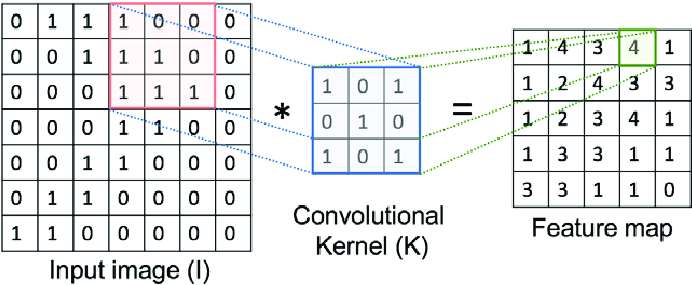
\includegraphics[width=0.6\linewidth]{conv.png} \caption{Συνέλιξη της εικόνας I με το φίλτρο K}
\label{figure:conv}  
\end{figure}


\subsubsection{Επίπεδο Υποδειγματοληψίας(Pooling layer)}
\label{subsubsec:3.1.3.2}


Το επίπεδο Υποδειγματοληψίας χρησιμοποιείται για τη μείωση της χωρικών διαστάσεων στους χάρτες χαρακτηριστικών και απαντάται κυρίως μετά από συνελεκτικά επίπεδα. Η μείωση των χωρικών διαστάσεων έχει σκοπό τη μείωση του αριθμού των παραμέτρων και των υπολογισμών. Επιπλέον, μειώνεται η πιθανότητα για  υπερεκπαίδευση. Οι δυο κύριες μέθοδοι υποδειγματοληψίας είναι η υποδειγματοληψία μεγίστου και η υποδειγματοληψία μέσου όρου. Στην πρώτη επιλέγεται η μέγιστη τιμή για ένα παράθυρο της εικόνας, ενώ στη δεύτερη υπολογίζεται ο μέσος όρος των τιμών του κάθε παραθύρου. Στην εικόνα \ref{figure:maxAvgPool} παρουσιάζονται οι  συνηθέστεροι μέθοδοι χωρικής υποδειγματοληψίας. Να σημειωθεί ότι το επίπεδο υποδειγματοληψίας εφαρμόζεται συνήθως στις διαστάσεις [ύψος x πλάτος] της εικόνας και όχι στη τρίτη διάσταση.



\begin{figure}[!h]
    \centering
      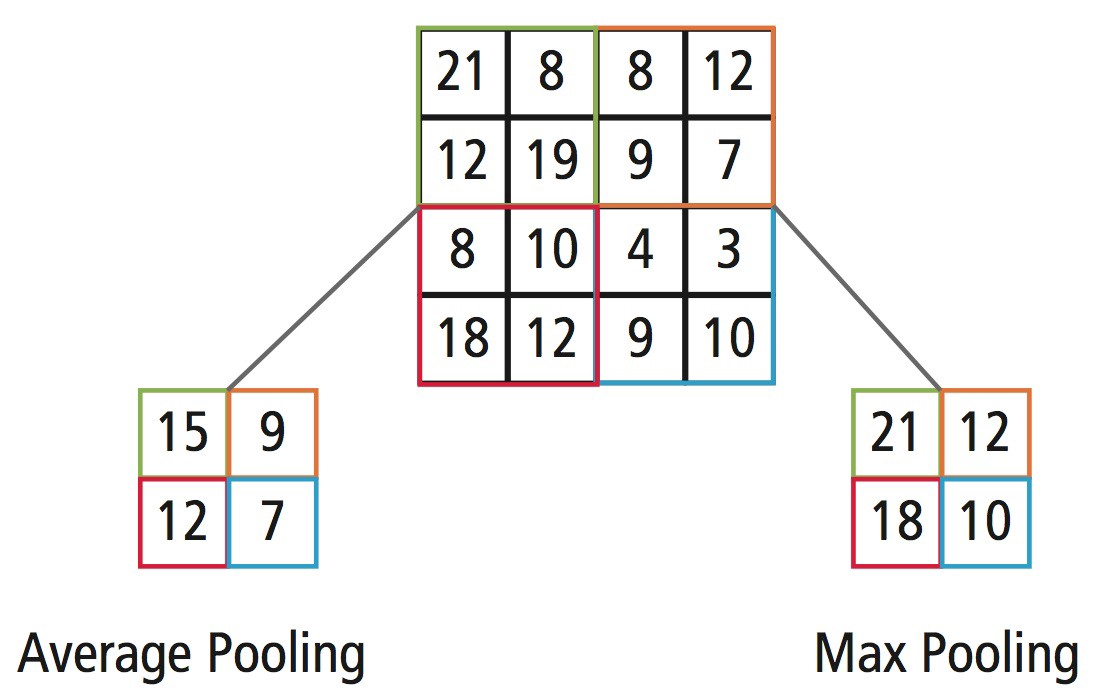
\includegraphics[width=0.6\linewidth]{maxAvgPool.jpeg} \caption{Υποδειγματοληψία μέσης (αριστερά) και μέγιστης (δεξιά) τιμής}
      \label{figure:maxAvgPool}    
  \end{figure}


\subsubsection{Καθολικό Επίπεδο Υποδειγματοληψίας(Global Pooling layer)}
\label{subsubsec:3.1.3.3}
Αποτελεί μία ειδική περίπτωση υποδειγματοληψίας καθώς ως παράθυρο υποδειγματοληψίας λαμβάνεται όλη η εικόνα. Όποτε, μία εικόνα με διαστάσεις (ύψος)x(πλάτος)x(κανάλια) μετατρέπεται σε (1)x(1)x(κανάλια). Συνήθως, χρησιμοποιείται μετά το τελευταίο συνελικτικό επίπεδο αντί της χρήσης ενός πλήρες συνδεδεμένου επιπέδου. Η πιο συνηθισμένη καθολική υποδειγματοληψία είναι η καθολική υποδειγματοληψία μέσου όρου που παρουσιάζεται στην εικόνα \ref{figure:gap2}



\begin{figure}[!h]
    \centering
      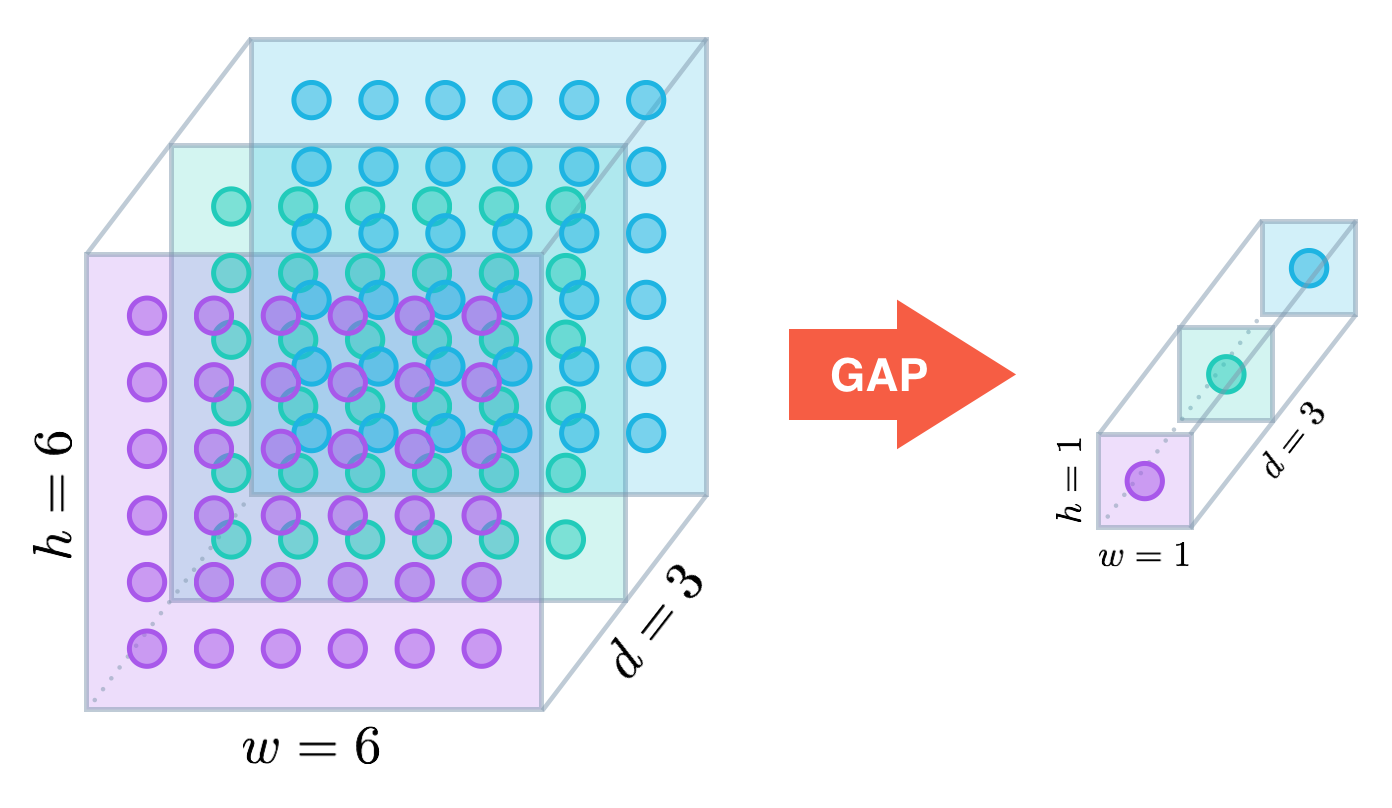
\includegraphics[width=0.6\linewidth]{gap2.png} \caption{Καθολική Υποδειγματοληψεία μέσου όρου}
      \label{figure:gap2}    
  \end{figure}


\subsubsection{Πλήρες Συνδεδομένο επίπεδο(Fully Connected Layer)}
\label{subsubsec:3.1.3.4}


Αποτελείται από  νευρώνες κάθε ένας εκ των οποίων συνδέεται με τους νευρώνες του προηγούμενου αλλά και του επόμενου πλήρους συνδεδεμένου επιπέδου(αν υπάρχουν). Συνήθως παρατηρείται μια ακολουθία από πλήρως συνδεδεμένα επίπεδα τα όποια τοποθετούνται πάντα μετά το τελευταίο συνελικτικό επίπεδο και αποτελούν το τελικό στάδιο για την ταξινόμηση των εικόνων. Το τελευταίο πλήρες συνδεδεμένο επίπεδο περιέχει τόσους νευρώνες όσες και οι κλάσεις του προβλήματος ταξινόμησης. Στην εικόνα \ref{figure:fullyconncted} παρουσιάζεται ένα πλήρες συνδεμένο επίπεδο.


\begin{figure}[!h]
    \centering
      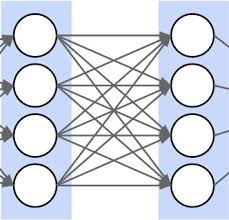
\includegraphics[width=0.2\linewidth]{fullyconncted.jpg} \caption{Πλήρες Συνδεδεμένο Επίπεδο}
\label{figure:fullyconncted}  
\end{figure}



\subsubsection{Επίπεδο Συνένωσης(Concatenate)}
\label{subsubsec:3.1.3.5}


Δέχεται εισόδους και τις συνενώνει κατά μήκος μιας συγκεκριμένης διάστασης. Οι είσοδοι πρέπει να έχουν το ίδιο μέγεθος εκτός από τη διάσταση που γίνεται η ένωση. Χρησιμοποιείται κυρίως μετά από παράλληλα επίπεδα ώστε να ενώσει τις εξόδους τους. Για παράδειγμα έστω οι εξής έξοδοι: $32x32x5$, $32x32x7$ και $32x32x5$. Η έξοδος του επίπεδου συνένωσης θα είναι $32x32x17$. Να σημειωθεί ότι αυτό το επίπεδο έχει περισσότερο προγραμματιστική υπόσταση και όχι τόσο λογική. Στην εικόνα \ref{figure:concat} παρουσιάζεται η συνένωση των εξόδων κάποιων παράλληλων επιπέδων.


\begin{figure}[!h]
    \centering
      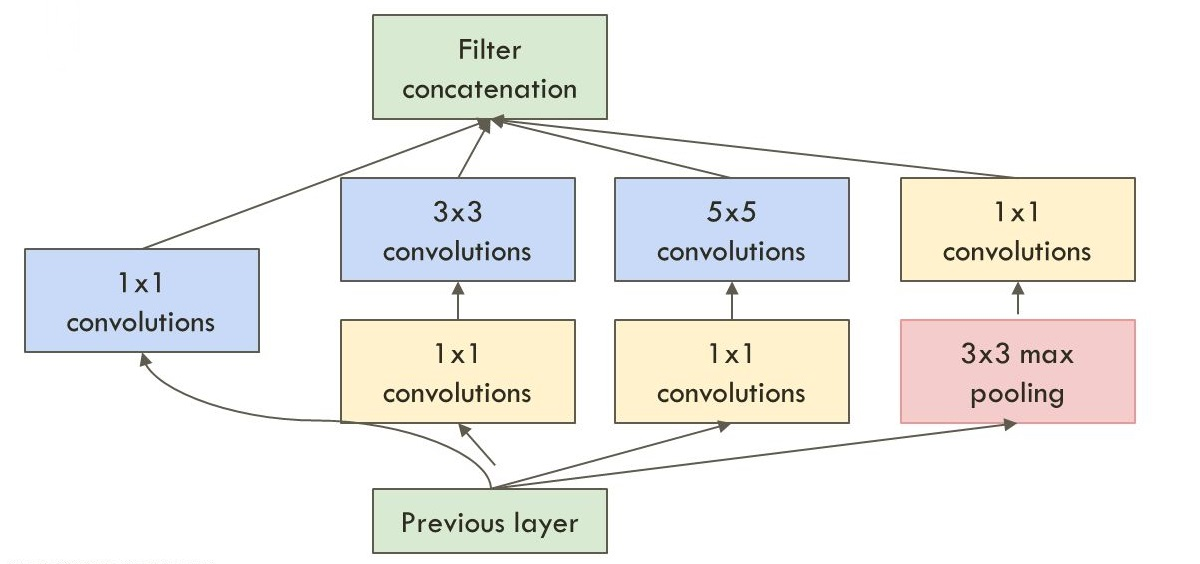
\includegraphics[width=0.8\linewidth]{concat.jpg} \caption{Συνένωση των εξόδων των φίλτρων στο επίπεδο Συνένωσης}
\label{figure:concat}  
\end{figure}


\subsubsection{Συνάρτηση Ενεργοποίησης(Activation Function) }
\label{subsubsec:3.1.3.6}


H συνάρτηση ενεργοποίησης αποφασίζει αν ένας νευρώνας πρέπει να ενεργοποιηθεί ή όχι. Σκοπός της συνάρτησης ενεργοποίησης είναι να εισάγει μη γραμμικότητα στη έξοδο ενός νευρώνα. Δύο από τις πιο συνηθισμένες συναρτήσεις ενεργοποίησης, που αναφέρθηκαν και πιο πάνω στα ANN, είναι η συνάρτηση Ανόρθωσης και η Σιγμοειδής συνάρτηση, οι οποίες παρουσιάζονται στις εικόνες \ref{figure:relu}, \ref{figure:sigmoid}. 





\begin{figure}[!h]
    \centering
      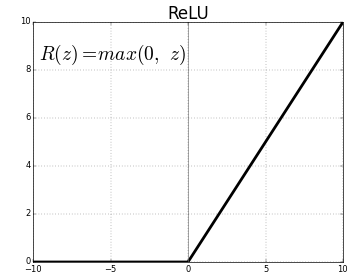
\includegraphics[width=0.5\linewidth]{relu.png} \caption{Συνάρτηση Ανόρθωσης}
      \label{figure:relu}    
  \end{figure}


\begin{figure}[!h]
    \centering
      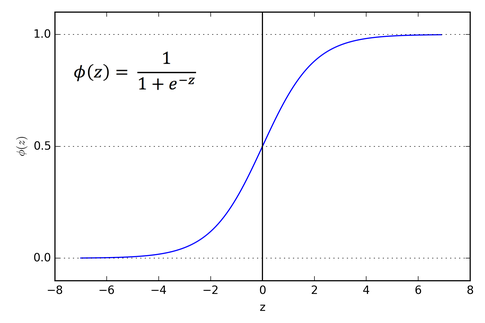
\includegraphics[width=0.5\linewidth]{sigmoid.png} \caption{Σιγμοειδής Συνάρτηση}
      \label{figure:sigmoid}    
  \end{figure}
  
\subsubsection{Επίπεδο Απόσυρσης(Dropout)}
\label{subsubsec:3.1.3.7}

Είναι μία τεχνική με σκοπό την μείωση της υπερεκπαίδευσης στα νευρωνικά δίκτυα. Υπερεκπαίδευση συμβαίνει όταν κατά τη διάρκεια της εκπαίδευσης το μοντέλο αποστηθίζει το σύνολο εκπαίδευσης με αποτέλεσμα να μην μπορεί να γενικεύσει. Έτσι, το μοντέλο αδυνατεί να προβλέψει σωστά την έξοδο για νέες εισόδους.
Κατά την εφαρμογή του επιπέδου Απόσυρσης, αγνοείται προσωρινά και με τυχαίο τρόπο κάποιο ποσοστό νευρώνων/φίλτρων τα οποία παράγουν μηδενική έξοδο και οι παράμετροι τους δεν ενημερώνονται. Το επίπεδο απόσυρσης εφαρμόζεται μόνο κατά τη διάρκεια της εκπαίδευσης. Έτσι, κατά τη διάρκεια της εκπαίδευσης, για κάθε επίπεδο που εφαρμόζεται απόσυρση, για κάθε είσοδο και για κάθε εποχή αγνοούνται κατά τυχαίο τρόπο κάποιο νευρώνες/φίλτρα. Στην εικόνα \ref{figure:dropout} παρουσιάζεται ένα πλήρες συνδεδεμένο δίκτυο χωρίς απόσυρση και το αντίστοιχο δίκτυο μετά την εφαρμογή απόσυρσης.


\begin{figure}[!h]
    \centering
      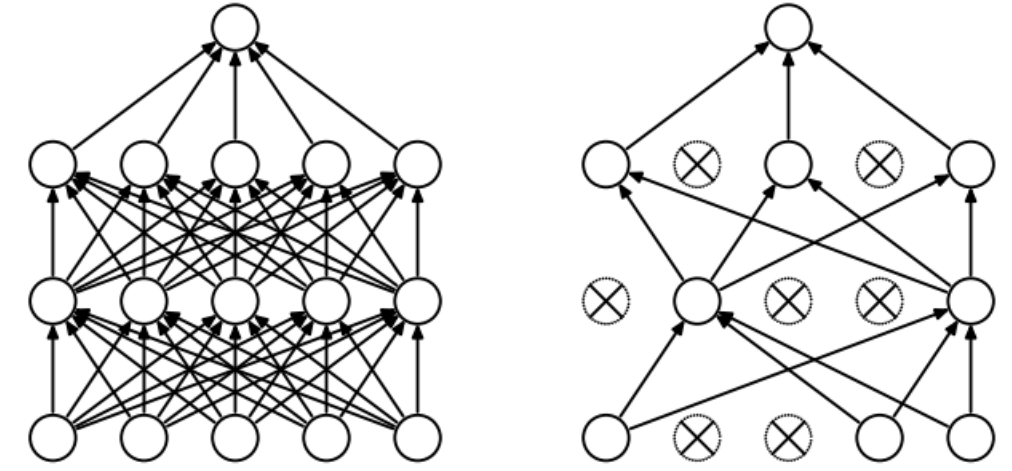
\includegraphics[width=0.8\linewidth]{dropout.png} \caption{Πλήρες συνδεδομένο δίκτυο χωρίς Dropout(αριστερά), με dropout(δεξιά)}
      \label{figure:dropout}    
  \end{figure}


\subsubsection{Κανονικοποίηση σε Πακέτα(Batch Normalization)}
\label{subsubsec:3.1.3.8}

Είναι μία τεχνική για βελτίωση της ταχύτητας, της επίδοσης και της σταθερότητας των CNN.\cite{BN}. Κατά τη διάρκεια της εκπαίδευσης ενός CNN, καθώς μεταβάλλονται οι παράμετροι των προηγούμενων επιπέδων, η κατανομή των εισόδων του τρέχοντος επιπέδου αλλάζει ανάλογα. Έτσι, το τρέχον επίπεδο πρέπει να αναπροσαρμόζεται συνεχώς σε νέες κατανομές. Ειδικότερα σε δίκτυα με πολλά επίπεδα το παραπάνω πρόβλημα είναι ακόμα πιο σοβαρό καθώς μικρές αλλαγές της κατανομής στα πρώτα επίπεδα θα ενισχυθούν καθώς διαδίδονται μέσα στο δίκτυο. Για τη μείωση αυτών των ανεπιθύμητων αλλαγών στις εισόδους κατά τη διάρκεια της εκπαίδευσης χρησιμοποιείται η κανονικοποίηση σε πακέτα. Η κανονικοποίηση δεν υφίσταται σε όλο το σύνολο δεδομένων αλλά σε μικρά υποσύνολα που ονομάζονται πακέτα. Επιπλέον, η τεχνική κανονικοποίησης σε πακέτα επιτρέπει τη χρήση υψηλότερου ρυθμού εκμάθησης(learning rate) ενώ συγχρόνως ρυθμίζει το δίκτυο έτσι ώστε να είναι ευκολότερη η γενίκευση και επομένως να μην είναι απαραίτητο να χρησιμοποιηθεί η τεχνική Απόσυρσης(dropout) για τη μείωση της υπερεκπαίδευσης.



Παρακάτω παρουσιάζονται τα βήματα που ακολουθούνται για τον υπολογισμό των νέων τιμών των εισόδων. Οι τιμές $\gamma$ και $\beta$ προσαρμόζονται από το δίκτυο κατά την διάρκεια της εκπαίδευσης.
 
 
\begin{algorithm}\captionsetup{labelfont={sc,bf}, labelsep=newline}
  \caption{Κανονικοποίηση σε πακέτα}\label{alg:the_alg}

\begin{algorithmic}

\State $Β \gets (x_{1},...x_{m})$

\State $μ_{Β}\gets \frac{1}{m}\sum_{i=1}^{m} x_{i} $

\State $σ_{Β}^2\gets \frac{1}{m} \sum_{i=1}^{m} (x_{i}- μ_{Β})^2$

\State $\hat{x_{i}} \gets \frac{x_{i}-μ_{Β}}{\sqrt(σ_{Β}^2 + ε)}$

\State $y_{i} \gets \gamma \hat{x_{i}} + \beta  \equiv BN_{\gamma, \beta}(x_{i}) $

\State return $y_{i}$
\end{algorithmic}
\end{algorithm}





\subsection{Support Vector Machine(SVM)}
\label{subsec:3.1.4}

To Support Vector Machine(SVM) είναι ένα μοντέλο για προβλήματα ταξινόμησης και παλινδρόμησης. \cite{svm} Μπορεί να λύσει τόσο  γραμμικά όσο και μη γραμμικά  προβλήματα. Ο αλγόριθμος δημιουργεί μία γραμμή ή ένα υπερεπίπεδο που χωρίζει τα δεδομένα στις επιθυμητές κλάσεις. Η δυσκολία του αλγορίθμου έγκειται στην εύρεση της βέλτιστης γραμμής ή υπερεπιπέδου για τη διαχωρισμό των δεδομένων.  

Στην \ref{figure:svm} οι κόκκινες και μπλε κουκίδες αναπαριστούν το σύνολο εκπαίδευσης ενώ τα X1 και X2 αποτελούν τα χαρακτηριστικά που περιγράφουν τα δεδομένα. Οι μπλε κουκίδες ανήκουν στην κλάση -1 ενώ οι κόκκινες στην κλάση +1. Να σημειωθεί ότι ενώ στην εικόνα \ref{figure:svm} τα δεδομένα περιγράφονται με δύο χαρακτηριστικά, στην πραγματικότητα τα δεδομένα συνήθως περιγράφονται από πολύ μεγαλύτερο αριθμό χαρακτηριστικών. Στην περίπτωση της παρούσας διπλωματικής τα χαρακτηριστικά των δεδομένων τα οποία εξάγονται από το πρώτο πλήρη συνδεδεμένο επίπεδο του νευρωνικού είναι 2048 ωστόσο μία τέτοια αναπαράσταση θα ήταν αδύνατη. Για ευκολότερη κατανόηση και μεγαλύτερη παραστατικότητα η παρακάτω ανάλυση του προβλήματος θα περιοριστεί σε προβλήματα δυαδικής ταξινόμησης δηλαδή διαχωρισμό των δεδομένων σε 2 κλάσεις.



\begin{figure}[!h]
    \centering
      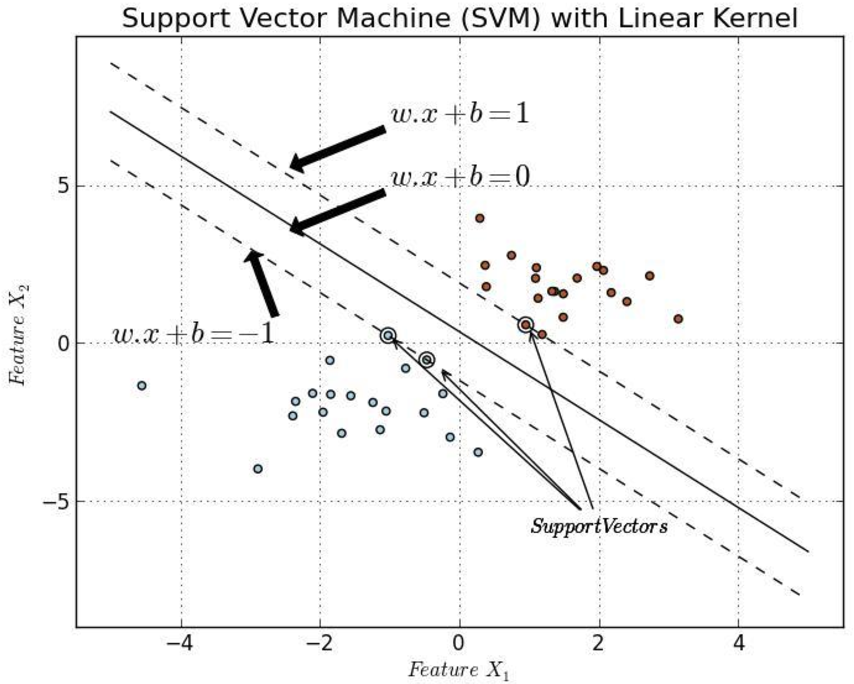
\includegraphics[width=0.8\linewidth]{svm2.png} \caption{Linear SVM}
\label{figure:svm}  
\end{figure}


Συνοπτικά, το πρόβλημα εύρεσης του βέλτιστου διαχωρισμού των δεδομένων μπορεί να τεθεί ως εξής. Έστω ένα σύνολο δεδομένων γραμμικά διαχωρίσιμο που κάθε δεδομένο ανήκει σε μία από τις δύο κλάσεις. Ο στόχος του αλγορίθμου είναι να μπορεί να  προβλέπει για νέα δεδομένα σε ποια κλάση ανήκουν. Αν θεωρήσουμε τα δεδομένα ως p-διαστατα διανύσματα, για το διαχωρισμό των δεδομένων πρέπει να βρεθεί ένα p-1 διαστατο υπερεπίπεδο. Για παράδειγμα για 2-διαστατα δεδομένα, αρκεί μία γραμμή για το διαχωρισμό τους ενώ για 3-διάστατα δεδομένα απαιτείται ένα επίπεδο(2D). Υπάρχουν πολλά υπερεπίπεδα που μπορούν να διαχωρίσουν τα δεδομένα ωστόσο ως βέλτιστο επιλέγεται το υπερεπίπεδο με το μεγαλύτερο περιθώριο μεταξύ των 2 κλάσεων. Έτσι, επιλέγεται το υπερεπίπεδο που η απόσταση από το πλησιέστερο δεδομένο κάθε κλάσης είναι μέγιστη. Αν αυτό το υπερεπιπεδο υπάρχει ονομάζεται\textit{ υπερεπίπεδο μέγιστου περιθωρίου} και ο γραμμικός ταξινομητής \textit{ταξινομητης μέγιστου περιθωρίου}. 



Αν το παραπάνω σύνολο  δεδομένων περιγραφεί  με σημεία της μορφής $(\vec{x}_{\,1},y_{1}),...,(\vec{x}_{\,n},y_{n})$, όπου τα $y_{i}$ είναι -1 ή 1 ανάλογα σε ποια κλάση ανήκουν τα $\vec{x}_{\,i}$ και τα $\vec{x}_{\,i}$ p-διάστατο διάνυσμα. Η περιοχή ανάμεσα στις δύο κλάσεις οριοθετείται από δύο υπερεπίπεδα και το  υπερεπιπεδο μεγίστου περιθωρίου που περιγράφηκε παραπάνω  βρίσκεται ανάμεσα στα δύο αυτά υπερεπίπεδα. Με ένα κανονικοποιημένο σύνολο δεδομένων, αυτά τα υπερεπίπεδα μπορούν να περιγραφούν με τις εξισώσεις \ref{eq:plane1}, \ref{eq:plane2}. Για την εξίσωση \ref{eq:plane1}, οτιδήποτε πάνω στο υπερεπίπεδο ή πάνω από το υπερεπίπεδο ανήκει στη κλάση 1 ενώ για την \ref{eq:plane2} οτιδήποτε πάνω στο υπερεπίπεδο ή κάτω από το υπερεπίπεδο ανήκει στη κλάση -1. 


\begin{equation} \label{eq:plane1}
\vec{w} \cdot  \vec{x} - b = 1
\end{equation}



\begin{equation} \label{eq:plane2}
\vec{w} \cdot  \vec{x} - b = -1
\end{equation}


Γεωμετρικά η απόσταση μεταξύ των δύο παραπάνω υπερεπιπέδων είναι $\frac{2}{||\vec{w}||}$. Επομένως, για να μεγιστοποιηθεί η απόσταση μεταξύ των υπερεπιπέδων, πρέπει να ελαχιστοποιηθεί το $||\vec{w}||$. Επιπλέον, πρέπει να ληφθούν υπόψη οι περιορισμοί \ref{eq:eq1} και \ref{eq:eq2}, ώστε τα δεδομένα  να μην βρίσκονται μέσα στο περιθώριο.


\begin{equation} \label{eq:eq1}
\vec{w}\cdot \vec{x}_{\,i} - b >= 1, ~αν ~y_{i} = 1
\end{equation}


\begin{equation} \label{eq:eq2}
\vec{w} \cdot \vec{x}_{\,i} - b <= 1, ~αν ~y_{i} = -1
\end{equation}
\\
\\
Τελικά, το πρόβλημα μπορεί να περιγραφεί ως εξής:


\begin{equation} \label{eq:eq3}
Minimize~||\vec{w}|| ~ for ~ y_{i}(\vec{w}\cdot \vec{x}_{\,i} - b)>= 1 για ~ i = 1,...,n
\end{equation}
\\


Μέσω της \ref{eq:eq3} υπολογίζονται τα $\vec{w}$ και $b$ τα οποία αρκούν για την περιγραφή του ταξινομητή. Η παραπάνω ανάλυση περιγράφει τη βασική λογική του αλγορίθμου, ωστόσο όταν τα δεδομένα δεν είναι γραμμικά διαχωρίσιμα, δηλαδή δεν μπορούν να διαχωριστούν από ένα υπερεπίπεδο, κάποια δεδομένα θα ταξινομούνται λάθος. Για αυτές τις περιπτώσεις ορίζεται μία επέκταση του SVM. Για την περιγραφή του νέου προβλήματος γίνεται χρήση της συνάρτησης hinge loss:
\\


\begin{equation} \label{eq:eq4}
max(0,1-y_{i}(\vec{w} \cdot \vec{x}_{\,i} - b))
\end{equation}
όπου η $ y_{i}$ είναι η πραγματική κλάση που ανήκει το $\vec{x_{\,i}}$ και $\vec{w} \cdot \vec{x}_{\,i}-b$ είναι η έξοδος του αλγορίθμου για το $\vec{x_{\,i}}$.


Η συνάρτηση είναι $0$, αν το $\vec{x_{\,i}}$ έχει ταξινομηθεί στη σωστή κλάση καθώς ο όρος $y_{i}(\vec{w}*\vec{x}_{\,i}-b)$ είναι πάντα μεγαλύτερος ή ίσος του 1 για σωστή ταξινόμηση του $\vec{x_{\,i}}$ οπότε το $1-y_{i}(\vec{w} \cdot \vec{x}_{\,i}-b)$ θα παίρνει τιμές μικρότερες ή ίσες το μηδενός. Ενώ όταν το $\vec{x_{\,i}}$ ταξινομηθεί σε λάθος κλάση, δηλαδή βρεθεί στη λάθος πλευρά του περιθωρίου,
 ο όρος $1-y_{i}(\vec{w} \cdot \vec{x}_{\,i}-b)$ θα παίρνει θετικές τιμές ανάλογες της απόστασης από το περιθώριο. Το πρόβλημα ελαχιστοποίησης  αναδιατυπώνεται ως εξής:


\begin{equation} \label{eq:eq5}
\frac{1}{n}  \sum_{i=1}^{n} max(0,1-y_{i}(\vec{w} \cdot \vec{x}_{\,i} - b))] + \lambda \cdot  ||\vec{w}||^2
\end{equation}
όπου η παράμετρος λ ορίζει το συμβιβασμό μεταξύ αύξησης περιθωρίου με παράλληλη μείωση των σωστών ταξινομήσεων.



Στην παρούσα διπλωματική εκτός του γραμμικού ταξινομητή, χρησιμοποιείται και ένας μη γραμμικός ταξινομητής με συνάρτηση πυρήνα την Gaussian Radial Basis η οποία περιγράφεται από την εξίσωση \ref{eq:eq7}. Για τη χρήση μη γραμμικών ταξινομητών ο  SVM χρησιμοποιεί μια συνάρτηση πυρήνα για να απεικονίσει το σύνολο δεδομένων σε ένα υψηλότερης διάστασης χώρο με σκοπό να γίνει γραμμικό σύνολο δεδομένων.


\begin{equation} \label{eq:eq7}
k(\vec{x}_{\,i},\vec{x}_{\,j}) = \exp(-\gamma ||\vec{x}_{\,i}- \vec{x}_{\,j} ||^2) ~ για ~ \gamma>0
\end{equation}



\section{Inception V3}
\label{sec:3.2}


Το Inception V3\cite{Szegedy} το οποίο χρησιμοποιήθηκε στην παρούσα διπλωματική αποτελεί ένα ευρέως χρησιμοποιούμενο συνελικτικό δίκτυο. Η αρχιτεκτονική Inception στην οποία ανήκει και το νευρωνικό Inception V3 αποτελείται από τις εξής εκδόσεις: Inception V1, Inception V2, Inception V3,Inception v4 και Inception-ResNet. Κάθε επόμενη έκδοση περιέχει βελτιώσεις στην επίδοση και στην ακρίβεια σε σχέση με την προηγούμενη. Ωστόσο, είναι δυνατόν μία παλαιότερη έκδοση να επιφέρει καλύτερα αποτελέσματα σε ένα  συγκεκριμένο σύνολο δεδομένων, σε σχέση με μία πιο καινούρια.


Η αρχιτεκτονική Inception αποτελεί ορόσημο για την ανάπτυξη των συνελικτικών δικτύων. Πριν από αυτή, τα πιο αποτελεσματικά CNN αύξαναν τα συνελικτικά επίπεδα πηγαίνοντας σε όλο και σε πιο βαθιες αρχιτεκτονικές, επιδιώκοντας καλύτερη επίδοση.


Στην αρχιτεκτονική Inception δεν ακολουθήθηκε η ίδια λογική, δηλαδή προσθήκη όλο και περισσότερων συνελικτικών επιπέδων αλλά προτάθηκε μία αρκετά πιο περίπλοκη δομή η οποία είναι αποτέλεσμα ιδεών που αναπτύχθηκαν από πολλούς ερευνητές κατά τη διάρκεια των προηγούμενων ετών.
Στην εικόνας \ref{figure:incV32} αποτυπώνεται η δομή του νευρωνικού Inception V3.


\begin{figure}[!h]

    \centering
      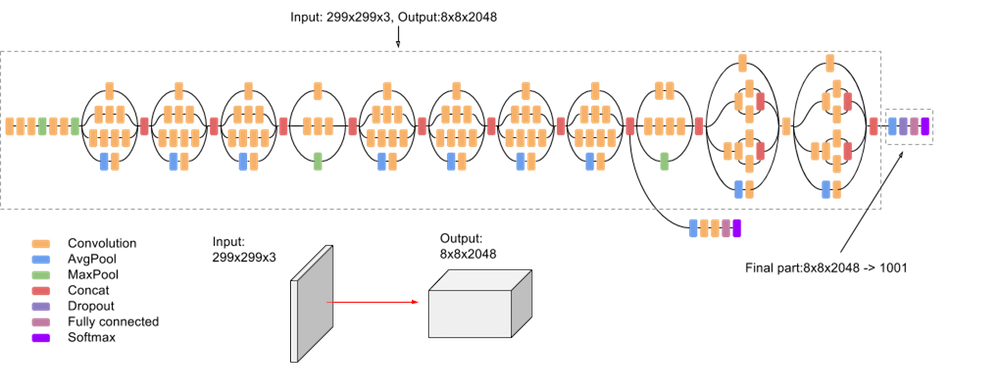
\includegraphics[width=1\linewidth]{incV3_2.png} \caption{Αρχιτεκτονική του νευρωνικού Inception V3}      
      \label{figure:incV32}  

  \end{figure}
  
  
\subsection{Τεχνικές σχεδίασης Inception V3}
\label{subsec:3.3.2}
Παρακάτω θα παρουσιαστούν οι κυριότερες τεχνικές σχεδίασης που προτάθηκαν στο Inception V3, ως μία βελτίωση των προηγούμενων εκδόσεων.


\subsubsection{Παραγοντοποίηση σε μικρότερα συνελικτικά επίπεδα}
\label{subsubsec:3.3.2.1}
Συνελίξεις με μεγαλύτερα χωρικά φίλτρα(πχ $5x5$ ή $7x7$) τείνουν να είναι δυσανάλογα ακριβές στους υπολογισμούς. Ένα συνελικτικό επίπεδο $5x5$ είναι 2.78 φορές πιο ακριβό υπολογιστικά σε σχέση με ένα $3x3$, με τον ίδιο αριθμό φίλτρων. Ωστόσο, στο $5x5$ συνελικτικό επίπεδο παρέχει μεγαλύτερη εκφραστικότητα. Για να είναι δυνατή η μείωση των παραμέτρων χωρίς όμως μείωση της ακρίβειας, προτείνεται η αντικατάσταση του φίλτρου $5x5$, χρησιμοποιώντας δύο συνελικτικα επίπεδα με $3x3$ φίλτρα και ίδιο αριθμό φίλτρων. Σε αυτή την περίπτωση ο αριθμός των παραμέτρων μειώνεται κατά $\frac{9+9}{25} = 28\%$. Στην εικόνα \ref{figure:a1} παρουσιάζεται ένα τμήμα του δικτύου, πριν και μετά την αντικατάσταση. Η παραπάνω αντικατάσταση μπορεί να γενικευθεί και για φίλτρα μεγαλύτερων διαστάσεων από $5x5$ , με αντικατάσταση αντίστοιχων $3x3$ επιπέδων.


\begin{figure}[!h]
\centering
\begin{subfigure}{.5\textwidth}
  \centering
  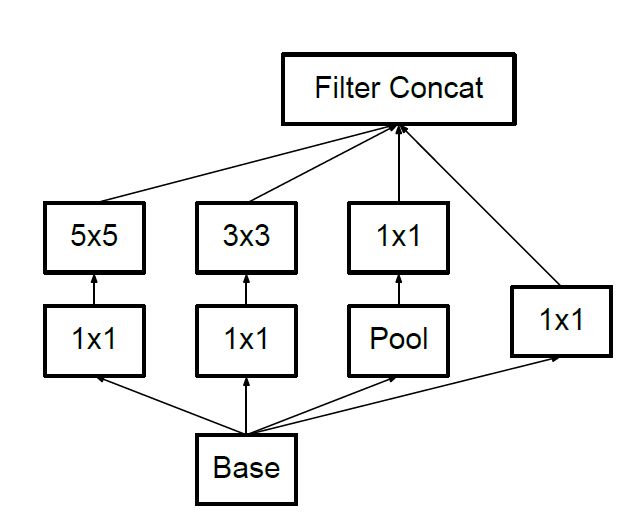
\includegraphics[scale=0.5]{0incV3.PNG}
  \caption{Αρχική δομή}
  \label{fig:sub11}
\end{subfigure}
\begin{subfigure}{.5\textwidth}
  \centering
  \includegraphics[scale=0.5]{1incV3.PNG}
  \caption{Μετά την αντικατάσταση}
  \label{fig:sub21}
\end{subfigure}
\caption{Αντικατάσταση του επιπέδου 5x5, με δύο 3x3 επίπεδα}
\label{figure:a1}
\end{figure}



\subsubsection{Παραγοντοποίηση σε μικρότερα μη συμμετρικά συνελικτικά επίπεδα}
\label{subsubsec:3.3.2.2}
Όπως παρουσιάστηκε και στην προηγούμενη παράγραφο ένα επίπεδο με φίλτρα μεγαλύτερων από $3x3$ διαστάσεων, μπορούν να αντικατασταθούν με μία  
αλληλουχία  επιπέδων με φίλτρα διαστάσεων $3x3$ και ίδιο αριθμό φίλτρων. Ωστόσο, τίθεται το ερώτημα, αν τα φίλτρα $3x3$ μπορούν να παραγοντοποιηθούν σε περισσότερα επίπεδα με μικρότερες διαστάσεις φίλτρων. Μία σκέψη θα ήταν να μετατραπούν σε δύο επίπεδα με $2x2$ φίλτρα, ωστόσο όπως αποδείχθηκε πειραματικά η παραγοντοποίηση σε ασύμμετρες συνελίξεις μπορεί να επιφέρει καλύτερα αποτελέσματα ενώ συγχρόνως επιφέρει μεγαλύτερη μείωση των παραμέτρων. Για παράδειγμα, έστω, φίλτρο διαστάσεων 3x3. Συνολικά, για αυτό το φίλτρο θα είχαμε $3*3 = 9$ παραμέτρους. Έστω τώρα ότι γίνεται αντικατάσταση του φίλτρο 3x3, με δύο φίλτρα  διαστάσεων 3x1 και 1x3. Συνολικά, τα 2 φίλτρα έχουν $3*1 + 1*3 = 6$ παραμέτρους. Ο αριθμός των παραμέτρων μειώθηκε κατά $33\%$. Αν αντίθετα, προτιμούνταν η χρήση $2$ συλλεκτικών επιπέδων με διάσταση φίλτρων $2x2$ τότε οι παράμετροι θα μειωνόταν κατά $\frac{2(2+2)}{3 \cdot 3}= 11\%$. Γενικά, η παραπάνω ανάλυση μπορεί να γενικευθεί για $nxn$ φίλτρα με αντικατάσταση από $1xn$ φίλτρα και $nx1$ φίλτρα. Στην εικόνα  \ref{figure:b2} παρουσιάζεται η παραπάνω αντικατάσταση.


\begin{figure}[!h]
\centering
\begin{subfigure}{.5\textwidth}
  \centering
  \includegraphics[scale=0.5]{1incV3.PNG}
  \caption{Αρχική δομή}
  \label{fig:sub1b2}
\end{subfigure}
\begin{subfigure}{.5\textwidth}
  \centering
  \includegraphics[scale=0.5]{2incV3.PNG}
  \caption{Μετά την αντικατάσταση}
  \label{fig:sub2b2}
\end{subfigure}
\caption{Αντικατάσταση κάθε επιπέδου 3x3, με ένα επίπεδο 1xn και ένα nx1}
\label{figure:b2}
\end{figure}


\subsubsection{Βοηθητικός Ταξινομητης}
\label{subsubsec:3.3.2.3}
Σε αντίθεση με προηγούμενες εκδόσεις της αρχιτεκτονικής Inception που χρησιμοποιήθηκαν 2 βοηθητικοί ταξινομητές στο Inception V3 χρησιμοποιήθηκε ένας μόνο βοηθητικός ταξινομητής στο τελευταίο $17x17$ συνελικτικό επίπεδο. Σε σχέση με τις προηγούμενες εκδόσεις που ο σκοπός των βοηθητικών ταξινομητών ήταν να επιτρέψουν πιο μεγάλο βάθος στο δίκτυα, ο σκοπός του βοηθητικού ταξινομητή στο Inception V3 είναι η χρήση του ως ρυθμιστή(regularizer) του δικτύου. Για την παρούσα διπλωματική παραλήφθηκε ο βοηθητικός ταξινομητής.


\subsubsection{Αποτελεσματική μείωση των διαστάσεων των χαρτών χαρακτηριστικών}
\label{subsubsec:3.3.2.4}
Για τη μείωση των διαστάσεων των χαρτών χαρακτηριστικών συνήθως χρησιμοποιείται μια συνάρτηση υποδειγματοληψίας. Επιπλέον, πριν την εφαρμογή του επιπέδου υποδειγματοληψίας τα κανάλια των χαρτών χαρακτηριστικών συχνά αυξάνονται με την εφαρμογή ενός συνελικτικού επιπέδου. 


Οπότε για να μειώσουμε τις διαστάσεις των χαρτών χαρακτηριστικών από k φίλτρα διαστάσεων dxd, σε $2k$ φίλτρα διαστάσεων $\frac{d}{2} x \frac{d}{2}$ πρέπει πρώτα να εφαρμοστεί ένα συνελικτικό επίπεδο με $2k$ φίλτρα και στη συνέχεια ένα επίπεδο υποδειγματοληψίας για την μείωση των διαστάσεων. Οι συνολικοί υπολογισμοί για τα παραπάνω είναι $2d^2 k^2$ και είναι ασύμφοροι λόγω της χρήσης συνελικτικού επιπέδου πριν τη μείωση των διαστάσεων. Αν γίνει αλλαγή στη σειρά του συνελικτικού επιπέδου και του επιπέδου υποδειγματοληψίας καταλήγουμε σε $\frac{d}{2}^2 k^2$, μειώνοντας το κόστος κατά $\frac{1}{4}$. Αυτός ο τρόπος δεν είναι ο πλέον αποδοτικός καθώς μειώνεται η διάσταση της αναπαράστασης σε $(d/2)^2 k$, καταλήγοντας σε μείωση της εκφραστικότητας του δικτύου. Αντί να γίνουν τα παραπάνω στο Inception V3 προτείνεται η χρήση δύο παράλληλων blocks: των P και C, το P είναι ένα επίπεδο υποδειγματοληψίας με παράθυρο $2x2$ και το C ένα συνελικτικό επίπεδο με ίδιο αριθμό φίλτρων με τον αρχικό χάρτη χαρακτηριστικών. Να σημειωθεί ότι το συνελεκτικό επίπεδο παράγεται με βήμα δύο, το οποίο σημαίνει ότι κατά τη συνέλιξη το φίλτρο θα μετατοπίζεται πάνω στην εικόνα, προσπερνώντας κάθε φορά ένα εικονοστοιχείο και πηγαίνοντας στο επόμενο. Στην εικόνα \ref{figure:PC} παρουσιάζονται γραφικά τα παραπάνω.



\begin{figure}[!h]
\centering
\begin{subfigure}{.5\textwidth}
  \centering
  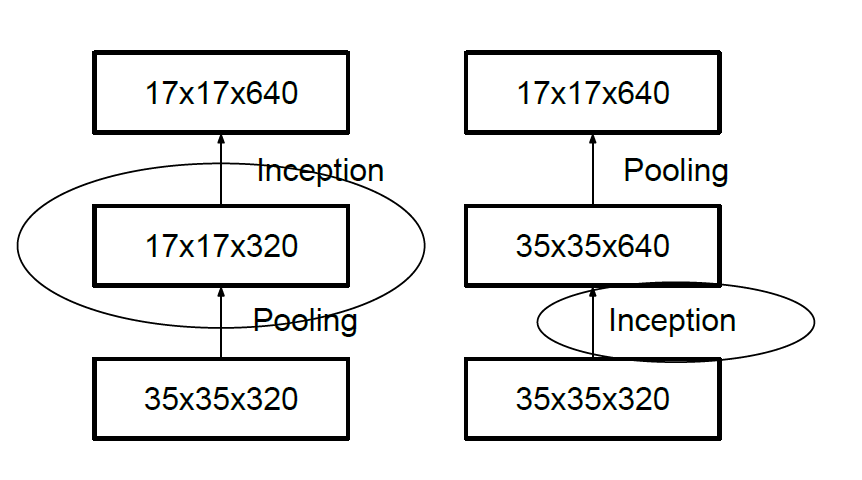
\includegraphics[scale=0.35]{expensive0incV3.PNG}
  \caption{Μη βέλτιστοι τρόποι μείωσης των διαστάσεων των χαρτών χαρακτηριστικών}
  \label{fig:sub1b}
\end{subfigure}%
\begin{subfigure}{.4\textwidth}
  \centering
  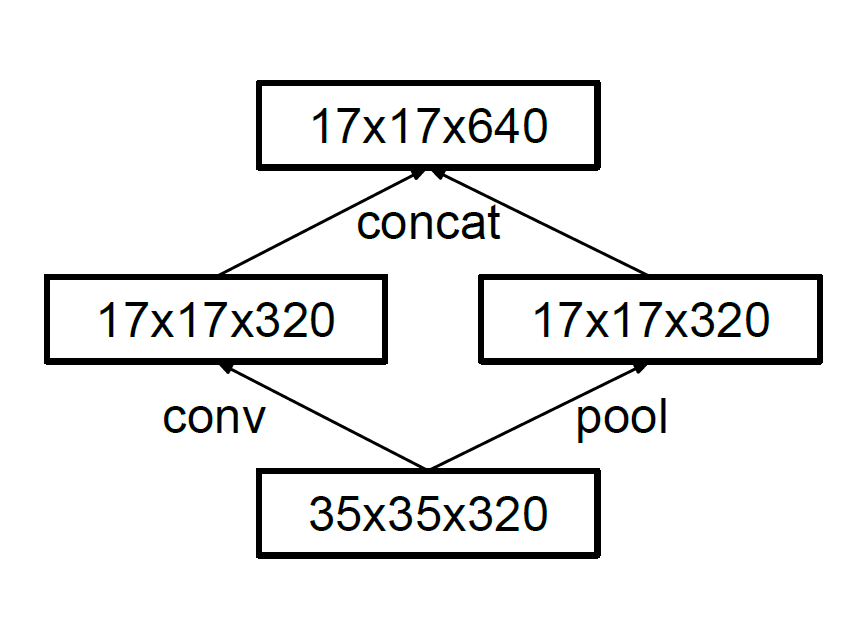
\includegraphics[scale=0.25]{3inv3.PNG}
  \caption{Βέλτιστος τρόπος μείωσης των διαστάσεων των χαρτών χαρακτηριστικών}
  \label{fig:sub2b}
\end{subfigure}
\caption{Μείωση των διαστάσεων των χαρτών Χαρακτηριστικών}
\label{figure:PC}
\end{figure}


\section{Εργαλεία}
\label{sec:3.4}
Το \textbf{matlab} είναι μία προγραμματιστική πλατφόρμα σχεδιασμένη ειδικά για μηχανικούς και ερευνητές με δυνατότητες ανάλυσης δεδομένων, ανάπτυξης αλγορίθμων, δημιουργίας μοντέλων και εφαρμογών. Στην παρούσα διπλωματική χρησιμοποιήθηκε κατά την διαδικασία επεξεργασίας των εικόνων, η οποία περιλαμβάνει την ανίχνευση του αμφιβληστροειδούς και τη μείωση των διαστάσεων των εικόνων.

Το \textbf{Tensorflow(TF)} είναι μία δωρεάν, ανοιχτού κώδικα βιβλιοθήκη, για μαθηματικούς υπολογισμούς. Χρησιμοποιείται σε πληθώρα εφαρμογών αλλά έχει καθιερωθεί για τη χρήση του σε Machine Learning εφαρμογές όπως Νευρωνικά Δίκτυα. Το TF μπορεί να τρέξει σε πολλαπλές CPUs και GPUs ενώ υποστηρίζει  64-bit Linux, mac OS, Windows, και πλατφόρμες κινητών όπως Android and iOS.


Το \textbf{Keras} είναι μία υψηλού επιπέδου βιβλιοθήκη νευρωνικών δικτύων γραμμένη σε Python. Μπορεί να τρέξει πάνω από TensorFlow, CNTK ή Theano.  Αναπτύχθηκε με γνώμονα τους γρήγορους υπολογισμούς και το γρήγορο πειραματισμό. Περιέχει υλοποιήσεις από αρκετά δομικά στοιχεία των νευρωνικών δικτύων. Επιπλέον, περιέχει έτοιμες υλοποιήσεις ευρέως διαδεδομένων νευρωνικών δικτύων.  Στην παρούσα διπλωματική επιλέχθηκε η χρήση της βιβλιοθήκης Keras πάνω σε Tensorflow για δημιουργία και εκπαίδευση των μοντέλων. Συνδυαστικά χρησιμοποιήθηκαν και άλλες πολλές βιβλιοθήκες της Python για διάφορους μετασχηματισμούς των εικόνων και για τη δημιουργία μοντέλων SVM.  


